\problemname{Sunset}

You are visiting a very warm country, and it happens to be a sizzling hot day. Luckily, you managed to find the shadow of a house to take cover in. You realize that you probably should head back to the hotel sometime soon, but you also realize that it's too hot to walk in the sun. The city you are in consists of $N$ houses, placed in a grid, where every house occupies exactly one unit square.

Currently, each house has a shadow that is exactly one unit square long, and is located directly north of the house. Since the sun just started to set, this shadow will extend one more unit square north per time unit. You can walk from the shadow of one house to another one, if the shadows share an edge of length at least one (see figure). You cannot walk through houses.

The question is how long it will take before there exists a path to the hotel that does not involve getting burned by the sun. The hotel is house number $N$, and you are currently in the shadow of house number 1. Since the hotel entrence is at the north side of the house, that's where you need to go. In the worst case you might have to wait until nightfall, which will occur in $K$ units of time.

\begin{figure}[ht!]
\centering
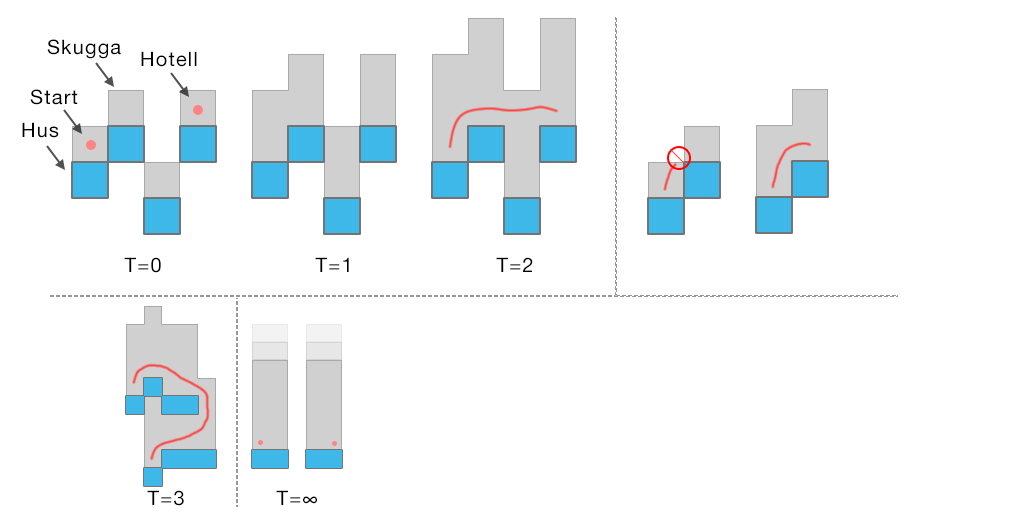
\includegraphics[width=0.6\textwidth]{skuggor.png}
\label{overflow}
\end{figure}

The first line contains two space-separated integers $N$ and $K$ - the number of houses in the city and the number of time units before nightfall.

The next $N$ lines contains 2 integers $x y$ each, the coordinates of the houses. The first line contains the coordinates of the house which you take cover behind, and the last line contains the coordinate of the hotel.

It is guaranteed that every house has a shadow, i.e. no house is placed immediately south of another house.

\section*{Output}
You should output a single integer, the time it takes before there exist a path to the hotell which goes entirely through the shadows, or \texttt{"NATT"} in case this time exceeds or equals $K$.

\section*{Scoring}
Your solution will be tested on a number of test case groups. To get points for a group
you have to solve all the test cases in that group.

\begin{tabular}{| l | l | l |}
	\hline
	Group & Points & Limits\\ \hline
	1 & 19 & $N, K \le 100, |x|, |y| \le 100$ \\ \hline
	2 & 26 & $N, K, |x|, |y| \le 1000$ \\ \hline
	3 & 17 & $N, K \le 1000, |x|, |y| \le 100000$ \\ \hline
	4 & 23 & $N \le 20000, K, |x|, |y| \le 10^7$ \\ \hline
	5 & 15 & $N \le 300000, K, |x|, |y| \le 10^{18}$ \\ \hline
\end{tabular}
